\subsection{Crossing BT}
\label{sec:Crossing-BT-impl}
    This tree is used for the main decision-making process. It is the third sub-tree to be executed, and the only one to be executed repeatedly.\\
    In multiple nodes we will use data about the detected vehicles, and collision parameters for each vehicle. Therefore, we first need to define the data structures used to store this information.\\\\
    \bfc{Vehicle data}\\
        The data structure for storing the information about the detected vehicles is defined as follows:
        \begin{lstlisting}[language=C++, caption={Vehicle data structure}, label={lst:vehicle_data}]
            struct vehicle_info {
                int id;
                double x_pos;
                double y_pos;
                double x_dot;
                double y_dot;
                double x_ddot;
                double y_ddot;
                double length;
                double width;
            };
            struct vehicles_data {
                int num_vehicles;
                std::vector<vehicle_info> data;
            };
        \end{lstlisting}
        The first struct \texttt{vehicle\_info} is used to store the information about single detected vehicle. The positions of the vehicles are expressed with relation to the robot frame, meaning the center of the robot is the origin of the coordinate system.\\
        The second struct \texttt{vehicles\_data} is used to store the information about all detected vehicles.\\\\
    \bfc{Collision data}\\
        The data structure for storing the collision parameters is defined as follows:
        \begin{lstlisting}[language=C++, caption={Collision data structure}, label={lst:collision_data}]
            struct collision_info {
                int car_id;
                double v_front;
                double v_back;
                bool collide;
            };
            struct collisions_data {
                int num_collisions;
                std::vector<collision_info> data;
            };
        \end{lstlisting}
        The first struct \texttt{collision\_data} is used to store the collision parameters for single vehicle.\\
        The \texttt{v\_front} and \texttt{v\_back} variables are the velocities of the robot to come into contact with the front or back of the vehicle. The figure \ref{fig:collision} shows the contact points we are calculating the velocities for.\\
        The \texttt{collide} variable is a boolean value that tells us if the robot is going to collide with the vehicle. It is calculated based on the current velocities of the robot and the vehicle.\\
        The second struct \texttt{collisions\_data} is used to store the information about all collisions.\\\\
    \bfc{Calculating the collision parameters}\\
        First, we need to state the assumptions we are making in order to simplify the calculation.\\
        The first assumption is about the coordinate system we are using. We are using the robot frame, where the robot's center is the system's origin, and all the positions are expressed in relation to this origin. The $x$-axis points forward, and the $y$-axis points to the left. We can assume this because the calculations are done periodically, and the results are only relevant for the current time step. It also simplifies the process, as the vehicle positions are already expressed in the robot frame.\\
        The second assumption is about the movement of the robot. We assume the robot is moving in a straight line with constant velocity. This is reasonable as we want the robot to be as predictable as possible, so we do not want to move the robot to the side. The assumption about the constant velocity, meaning the acceleration is zero, is also reasonable. The speeds the robot can achieve are much lower than the robot's acceleration, so that we can neglect the acceleration.\\
        The third assumprion is about the movement of the vehicle. We assume the vehicle's acceleration is constant. This is a reasonable simplification as the calculation is done periodically.\\
        The fourth assumption is that we will calculate the collision only in two dimensions. This is reasonable as we are only interested in the information if the collision will occur or not. Moreover, the area over which the collision can occur is relatively small, and therefore, any terrain deviation will not significantly impact the collision.\\\\
        Figure \ref{fig:collision} depicts a schematic view of the collision. There are two contact points, both on the robot and the vehicle. The first one (blue) is the point where the robot is going to collide with the front of the vehicle. The second one (red) is the point where the robot is going to collide with the back of the vehicle.\\
        \begin{figure}[ht]
            \centering
            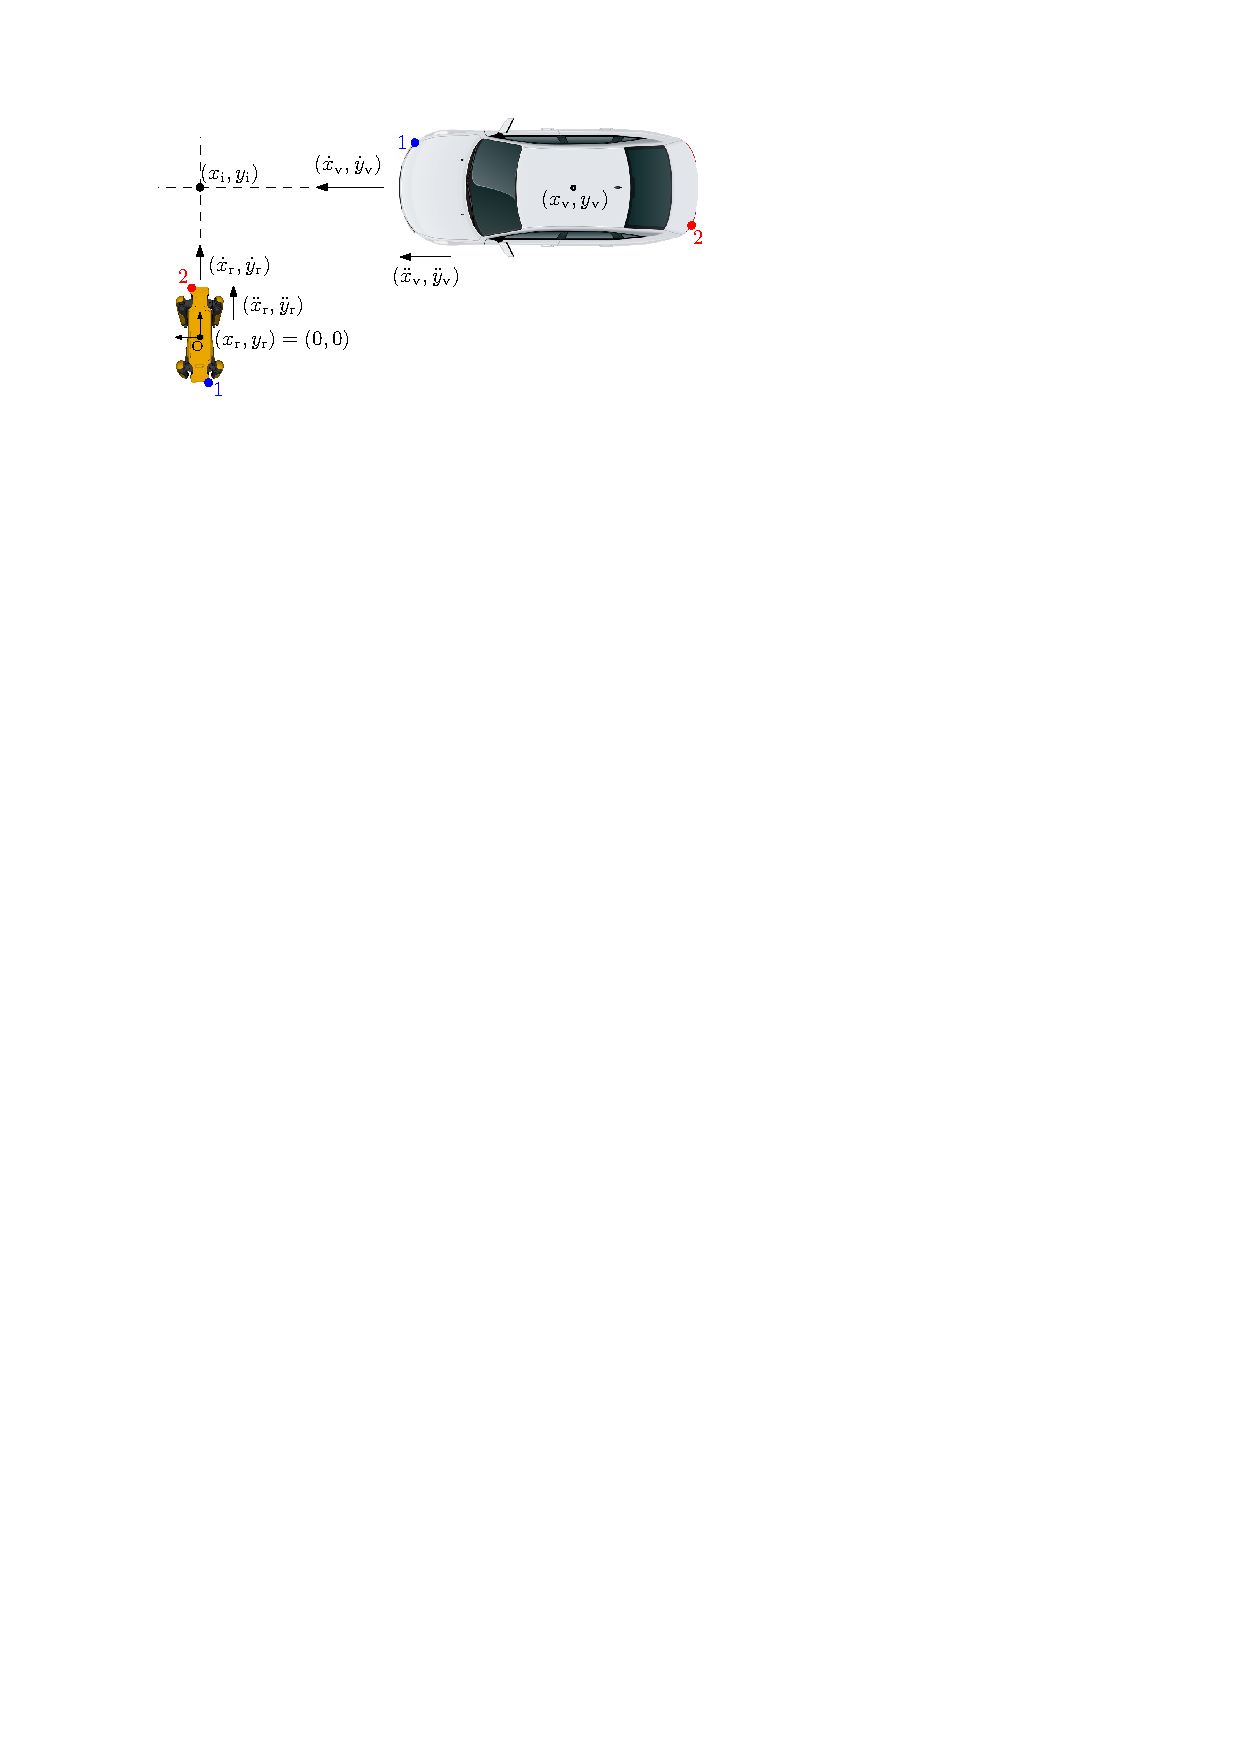
\includegraphics[height=6cm]{images/collision.pdf}
            \caption{Visualization of collision points, coordinate system, and vehicle parameters.}
            \label{fig:collision}
        \end{figure}
        \noindent For the first point, we calculate the velocity \texttt{v\_front}. This velocity depicts the minimal speed of the robot to cross in front of the vehicle. We calculate the velocity \texttt{v\_back} for the second point. This velocity depicts the maximal speed of the robot to cross behind the vehicle.\\
        The calculation is divided into three parts. In the first part, we determine the starting positions of the robot and the vehicle. In the second part, we calculate the time when the vehicle will reach the intersection point $(x_{\rm{i}}, y_{\rm{i}})$. In the last part, we calculate the velocities for the robot to collide with the vehicle.\\\\
        The first part is necessary as the coordinates of both the robot and the vehicle are at the center of their respective bodies. We need to move the starting points concerning the robot's and vehicle's length and width. The starting points for the robot are calculated using these equations:
        \begin{align}
            x_{\rm{r,f}} &= \frac{l_{\rm{r}}+w_{\rm{v}}}{2},\\
            x_{\rm{r,b}} &= \frac{l_{\rm{r}}+w_{\rm{v}}}{2},\\
            y_{\rm{r,f}} &= y_{\rm{r,b}} = 0,
        \end{align}
        where $l_{\rm{r}}$ is the length of the robot and $w_{\rm{v}}$ is the width of the vehicle.\\
        The starting points for the vehicle are calculated as follows:
        \begin{align}
            x_{\rm{v,f}} &= x_{\rm{v}} + \frac{l_{\rm{v}}+w_{\rm{r}}}{2}\cos{(\varphi_{\rm{v}})},\\
            x_{\rm{v,b}} &= x_{\rm{v}} - \frac{l_{\rm{v}}+w_{\rm{r}}}{2}\cos{(\varphi_{\rm{v}})},\\
            y_{\rm{v,f}} &= y_{\rm{v}} + \frac{l_{\rm{v}}+w_{\rm{r}}}{2}\sin{(\varphi_{\rm{v}})},\\
            y_{\rm{v,b}} &= y_{\rm{v}} - \frac{l_{\rm{v}}+w_{\rm{r}}}{2}\sin{(\varphi_{\rm{v}})},
        \end{align}
        where $\varphi_{\rm{v}} = \arctan{\left(\frac{\dot{y}_{\rm{v}}}{\dot{x}_{\rm{v}}}\right)}$ is the angle of the vehicle, $l_{\rm{v}}$ is the length of the vehicle and $w_{\rm{r}}$ is the width of the robot.\\
        We put the width of the robot to the calculation of the vehicle's starting points and vice versa because we want to flatten the dimensions of the objects. This is done to simplify the calculation of the intersection point of the robot's and vehicle's trajectory.\\
        The second part of the calculation is further divided into two parts. The reason is, that there are two possible scenarios for the calculation. We will use the general equation of motion \cite{equation_motion} for both calculations.\\
        In the first scenario, the vehicle's acceleration is the $y$-axis is zero. That means we can calculate the time using the following equations:
        \begin{align}
            t_{\rm{f}} = -\frac{y_{\rm{v,f}}}{\dot{y}_{\rm{v}}},\\
            t_{\rm{b}} = -\frac{y_{\rm{v,b}}}{\dot{y}_{\rm{v}}}.
        \end{align}
        In the second scenario, the acceleration of the vehicle in the $y$-axis is non-zero. This scenario is more probable, as vehicles rarely drive at a constant speed. In this case, the time is calculated in the following way:
        \begin{align}
            t_{\rm{f},1,2} = \frac{-\dot{y}_{\rm{v}}\pm\sqrt{\dot{y}_{\rm{v}}^2-2\ddot{y}_{\rm{v}}y_{\rm{v,f}}}}{\ddot{y}_{\rm{v}}},\\
            t_{\rm{b},1,2} = \frac{-\dot{y}_{\rm{v}}\pm\sqrt{\dot{y}_{\rm{v}}^2-2\ddot{y}_{\rm{v}}y_{\rm{v,b}}}}{\ddot{y}_{\rm{v}}}
        \end{align}
        There are two possible solutions for each time. The reason is that the vehicle may be decelerating and therefore change the direction of its travel. The interpretation of the results and the selection of the correct solution is discussed in the next section.\\
        The last part of the calculation is the calculation of the velocities. First, we need to calculate the position of the vehicle in the $x$-axis at the time of the collision. We use the general equation of motion with $t_{0}=0\:\rm{s}$:
        \begin{align}
            x_{\rm{i,f}} &= x_{\rm{v,f}} + \dot{x}_{\rm{v}}t_{\rm{f}} + \frac{1}{2}\ddot{x}_{\rm{v}}t_{\rm{f}}^2,\\
            x_{\rm{i,b}} &= x_{\rm{v,b}} + \dot{x}_{\rm{v}}t_{\rm{b}} + \frac{1}{2}\ddot{x}_{\rm{v}}t_{\rm{b}}^2.
        \end{align}
        Now we can calculate the velocities of the robot.
        \begin{align}
            \dot{x}_{\rm{r,f}} &= \frac{x_{\rm{i,f}}-x_{\rm{r,b}}}{t_{\rm{f}}},\\
            \dot{x}_{\rm{r,b}} &= \frac{x_{\rm{i,b}}-x_{\rm{r,f}}}{t_{\rm{b}}}.
        \end{align}
        The calculated velocities may be positive or negative. The interpretation is explained in the following section.\\\\
    \bfc{Interpretation of the calculated collision parameters}\\
        We will divide this section into two parts. The first part is the interpretation of the calculated time. The second part is the interpretation of the calculated velocities.\\\\
        If the calculated time is positive, the intersection point of the robot's and vehicle's trajectory is in the future. This means that the robot can collide with the vehicle without either of them changing the direction of travel.\\
        If the calculated time is negative, it means that the intersection point of the robot's and vehicle's trajectory is in the past. This means that the robot can collide with the vehicle, but only if the vehicle or the robot changes the direction of travel.\\
        The time can also be zero. This means that the robot and vehicle already collided. Therefore, we do not expect such a result to arise.\\
        We may have up to two solutions when calculating the times for non-zero acceleration. If we have none, the robot's and the vehicle's trajectories do not intersect.\\
        If we have one solution, the robot's and the vehicle's trajectories intersect only once. The interpretation is that the vehicle is decelerating and will stop at the intersection point and then start reversing.\\
        If we have two solutions, the robot's and the vehicle's trajectories intersect multiple times. Multiple intersections could have several physical interpretations. We can interpret this as the vehicle decelerating, and therefore, changing the direction of travel after passing the intersection point. We can also interpret this as the vehicle accelerating, and therefore, the second time of the intersection is likely negative.\\
        When choosing the calculated time, we will use the following criteria. If one time is positive and the second is negative, we will use the positive time. If both times are positive, we will use the shorter time. If both times are negative, we will use the larger time (the time that is closer to the present).\\\\
        The velocities can also be positive or negative. The interpretation is similar to the one of time. Positive velocity means moving forward, while negative velocity means moving backward.\\
        While it may seem irrelevant to calculate the time and velocity for backward movement, it is essential. The reason is that some other vehicle in front of the robot may be moving so that the robot collides with it. In this case, the robot will have to move backward to avoid the collision, and we need to be able to set the correct backward velocity to not collide with the first vehicle.
